In this section the results of the MPO construction detailed in

\subsection{Exact tensor matrix exponential } \label{chap_bench}

The performance of the MPO construction can be compared with the exact diagonalisation of the hamiltonian for a given number of sites. To obtain a faithful results, the number of sites should be as high as possible. In practice, diagonalisation of large matrices becomes slow and memory consuming. The size grows exponentially in the number of sites: $d^{n} \times d^{n} $. A double takes 8 bytes of memory.A Rough estimated of the amount of RAM $R$ needed to store this complex array is:

\begin{equation}
    R = d^{2 n} \times 16 bytes
\end{equation}

Which means a 14 site chain already takes up more than 4 GB of RAM. The complexity to calculate a matrix exponential scales as $O(n^3)$ \cite{Moler2003}. In practice this means that, without any tricks, the matrix exponential can be calculated for 12 sites.

State of the art algorithm for exact diagonalisation, which include all symmetries and are optimised for parallelisation, can calculate up to 50 sites. \cite{Wietek2018}

\subsubsection{Norms} \label{mponormdef}
\def \expHBlock {\expH{4}{ $e^{- \beta \hat{H}_{n}}$   }{ {,,"...",} }{ {,,"...",} }{}{} }
\def \Mn {\mpo{4}{ {0,,,,0}  }{}{}{{0,0,1,0,0}}{}}

The schatten 2 norm is used in the following analysis, denoted by ${\| \cdot \|} _{2}$. In the figures the relative error $\epsilon$ is reported.

\begin{equation}
    \epsilon = \frac{  {  \left \|  \expHBlock - \Mn  \right \|} _{2}  }{ {  \left\|  \expHBlock \right \|}_2}
\end{equation}

This norm can only be calculated for a finite number of sites. The influence of the number of sites for a linear  and cyclic \cref{benchmarking:systemsize}. As expected, the cyclic norm represents large systems better for the same number of sites. The linear norm keeps increasing with every added site.

Calculating the cyclic norm comes at the extra cost of contracting a cyclic tensor network. In this chapter, the cyclic norm will be given for M=11 sites.

\begin{figure}
    \begin{subfigure}[]{\linewidth}
        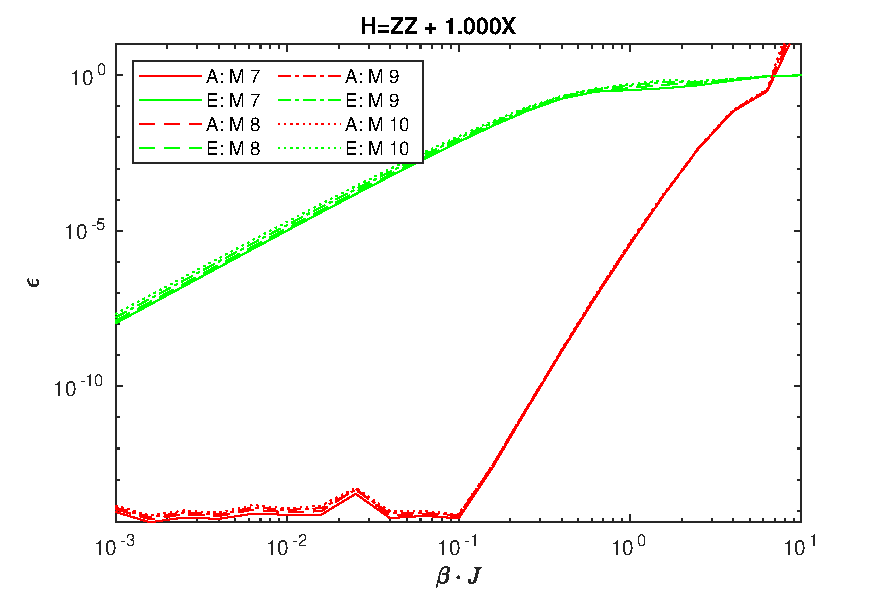
\includegraphics[width=\textwidth]{Figuren/benchmarking/comp_M_cycl.pdf}
        \subcaption{Cyclic error}
    \end{subfigure}
    \begin{subfigure}[]{\linewidth}
        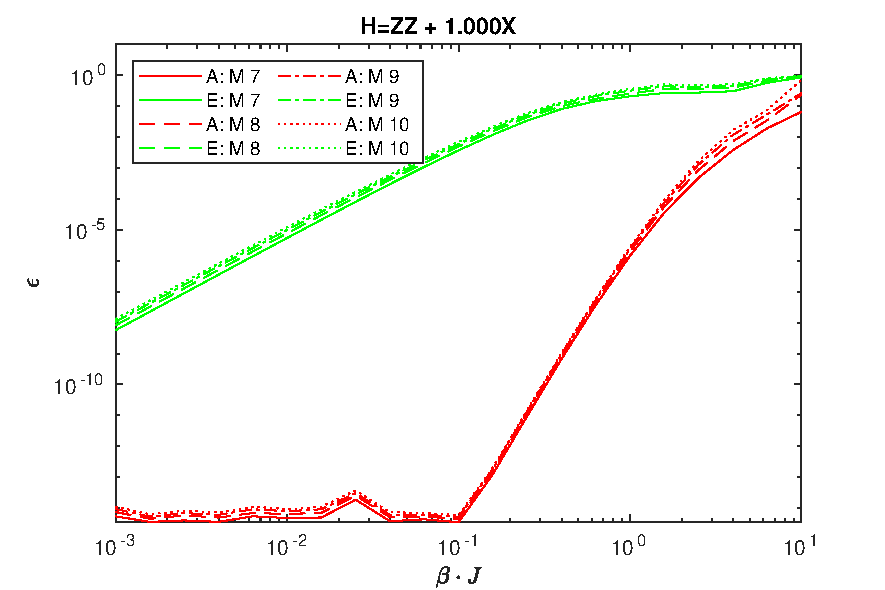
\includegraphics[width=\textwidth]{Figuren/benchmarking/Comp_M_lin.pdf}
        \subcaption{Linear error}
    \end{subfigure}
    \caption{ Different error measures for 1D transversal Ising model }
    \label{benchmarking:systemsize}
\end{figure}

\subsection{Inversion procedure}\label{subsec:inversion_procedure}

\subsubsection{Full pseudo-inversion}

The procedure for inversion of the linear blocks was detailed in \cref{subsec:linear_solver}. To demonstrate the need for a pseudoinverse, the error for transversal Ising models is shown in \cref{benc:fig:fullinv}. The pseudoinversion has 1 parameter $\sigma_0$, the cutoff below which the singular values are set to zero. A value of $10^{-12}$ seems optimal in the sense that it doesn't introduce large fluctuations, but still is able to produce good inverses.

\begin{figure}
    \center
    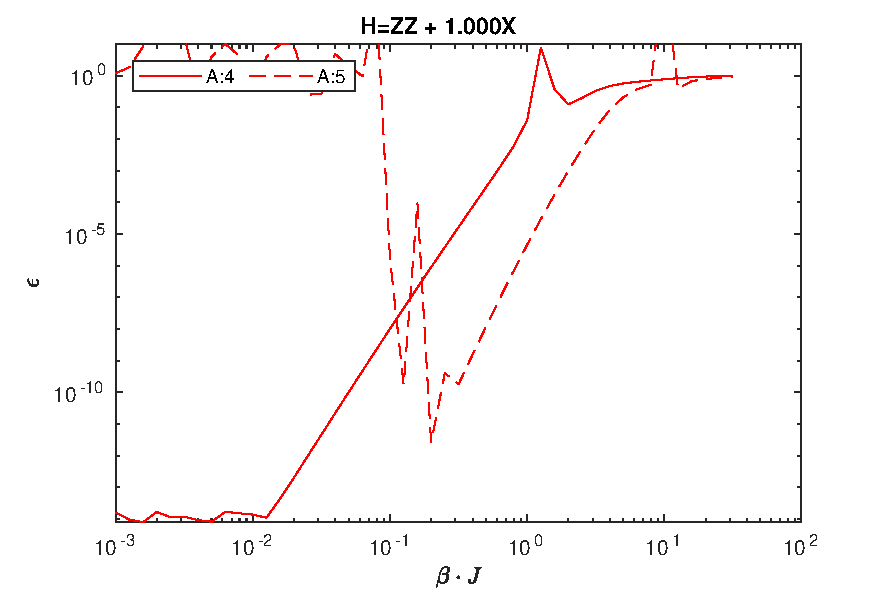
\includegraphics[width=\textwidth]{Figuren/benchmarking/t_ising_full_inverse.pdf }
    \caption{Error for transversal Ising, computed with full inversion }
    \label{benc:fig:fullinv}
\end{figure}

\paragraph{Truncation}

The original 1D code does not yet have this full inversion procedure. Instead, an optimality criterium was devised to truncate the series. Needless to say, even with this criterium, the results were a lot worse at low beta.

\subsection{Models}

With these basic definitions and findings out of the way, the different series expansions can be tested against some different physical models.

\subsubsection{Ising}

The results for the different types are all bundled in \cref{fig:benchmark:tising}. The vertical axis show the logarithm of the relative error $\epsilon$, horizontal axis the normalised inverse $beta= \frac{J}{T}$. The most surprising finding is the fact that the strict type E performs worse than the others. For low $\beta$, it is more than 5 orders of magnitude worse, Taken together with its large bond dimension, this expansion  and all other strict variants are seen to be of no use.

Now lets focus on the 2 other variants. Type A clearly outperforms type F for all $\beta<2$ by quite some margin. Only for large $\beta$, type F has the upper hand. While not completely clear in the picture, type A has quite a large error for some orders at $\beta \in (2,10) $, but higher orders seems to solve the problem. The construction of type F requires twice the bond dimension, and hence type A performs clearly better overal

\begin{figure}
    \center
    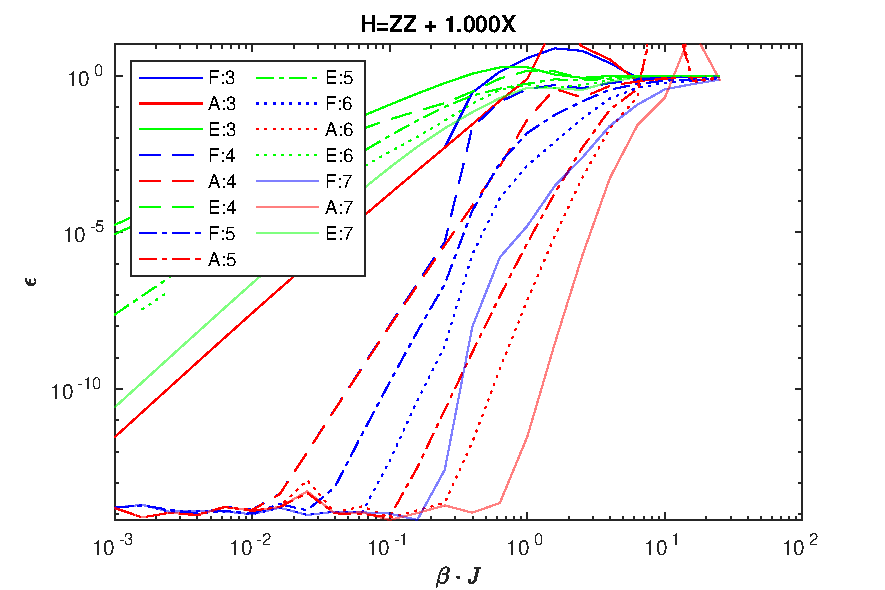
\includegraphics[width=\textwidth]{Figuren/benchmarking/t_ising.pdf}
    \caption{Comparison type A, E and F for Transversal Ising. }
    \label{fig:benchmark:tising}
\end{figure}

\subsubsection{Heisenberg}

Now we focus on the spin 1/2 Heisenberg model on a chain. The results are again displayed in \cref{fig:benchmark:tHeisenberg}. The exact type seems to perform a lot better here, but still has consistently the largest error of the 3 methods for a given order. For low $\beta$, type A again performs better than type F. At $\beta \approx 1$ and larger, F starts to improve upon the result of A, and doesn't have an divergent error.

\begin{figure}
    \center
    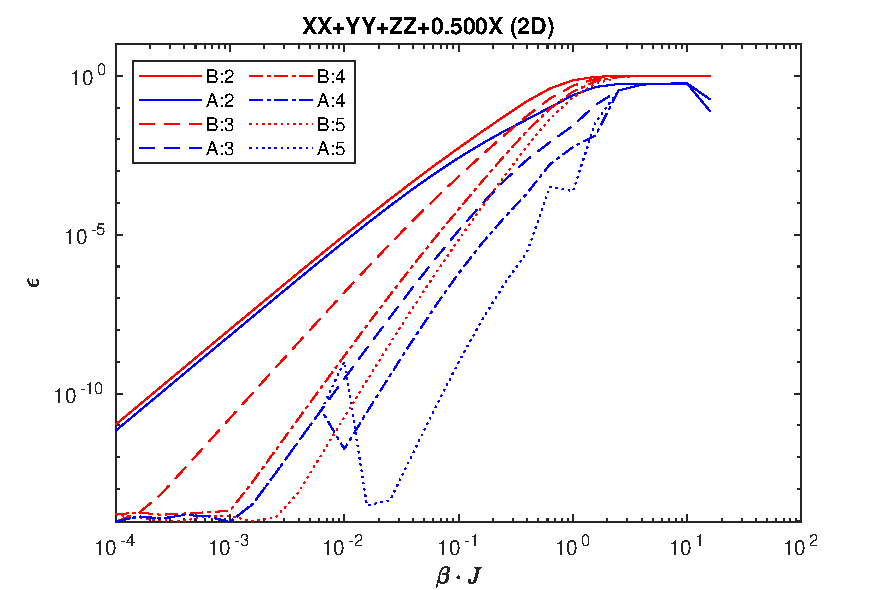
\includegraphics[width=\textwidth]{Figuren/benchmarking/t_heis_XXX.pdf}
    \caption{Comparison type A, E and F for Heisenberg model.}
    \label{fig:benchmark:tHeisenberg}
\end{figure}

\subsubsection{Random}

To give a representative overview for random hamiltonians, several simulations were run. The single site and nearest neighbour hamiltonians are generated by making hermitian matrices with random real and complex numbers between -1 and 1. In order to compare the different graphs, the energy scale is set such that the norm of the hamiltonian evaluated on 2 sites is 1.

\cref{fig:benchmark:trand} shows the results for 2 random hamiltonians. This is done to ensure that the chosen models are not too 'simple'. The results show once again that the strict variant performs worse than the other 2. In comparison to the previous models, Type F performs very well, especially at high $\beta$.

\begin{figure}
    \begin{subfigure}[]{\textwidth}
        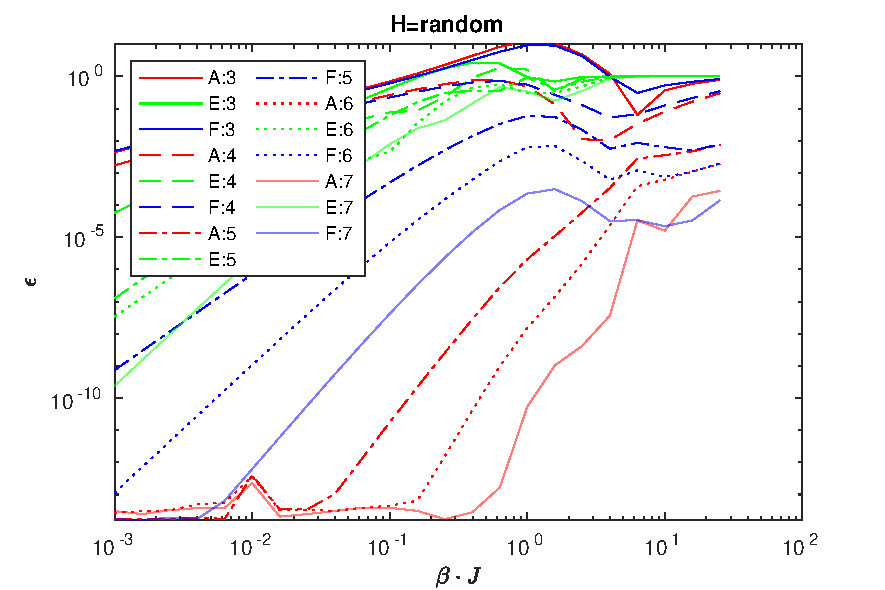
\includegraphics[width=\textwidth]{Figuren/benchmarking/1D_Raand.pdf}
        \subcaption{}
    \end{subfigure}

    \begin{subfigure}[]{\textwidth}
        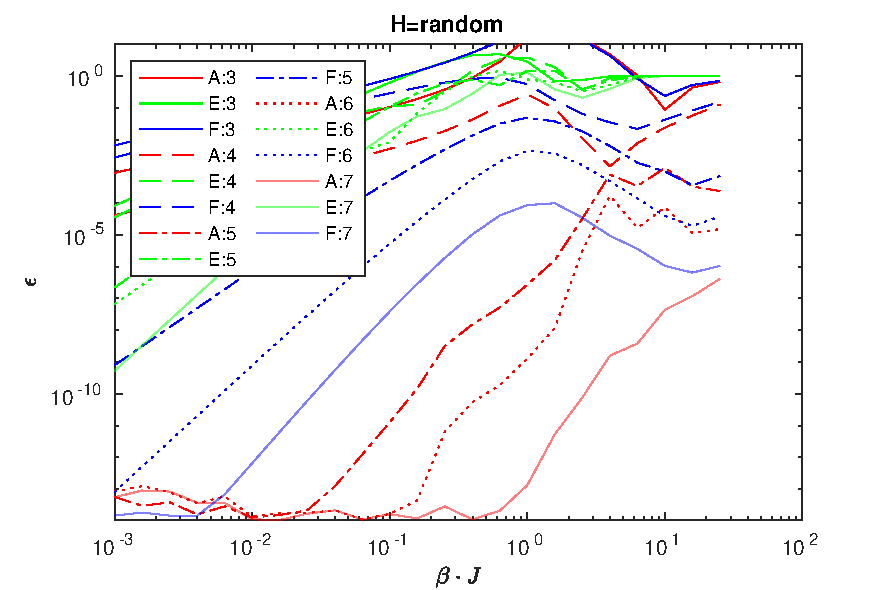
\includegraphics[width=\textwidth]{Figuren/benchmarking/1D_Raand_2.pdf}
        \subcaption{}
    \end{subfigure}

    \caption{Comparison type A, E and F for 2 random generated hamiltonians.}
    \label{fig:benchmark:trand}
\end{figure}

% \begin{figure}
%     \begin{subfigure}[]{\textwidth}
%         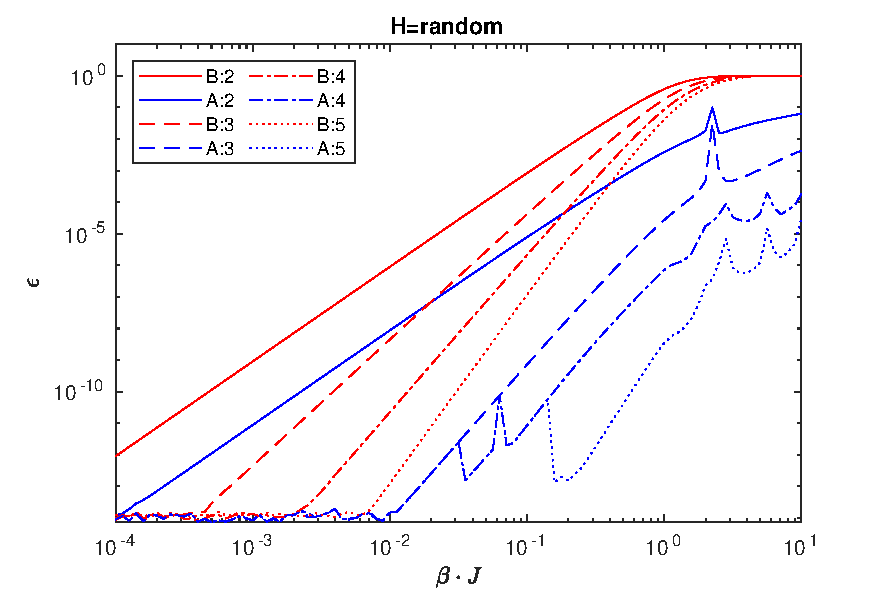
\includegraphics[width=\textwidth]{Figuren/benchmarking/rand_01.pdf}
%         \subcaption{test}
%     \end{subfigure}

%     \medskip

%     \begin{subfigure}[]{\textwidth}
%         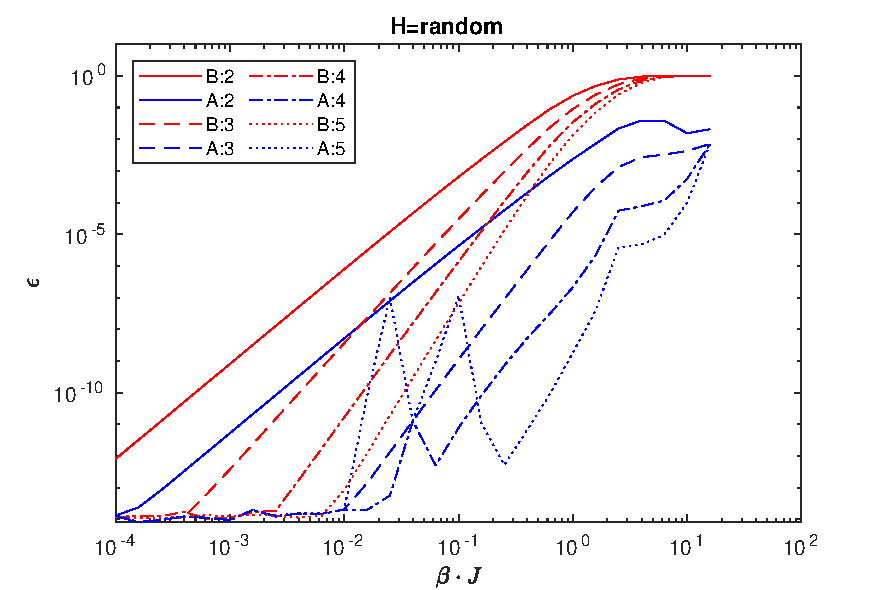
\includegraphics[width=\textwidth]{Figuren/benchmarking/rand_02.pdf}
%         \subcaption{test}
%         \label{benchmark:rand2}
%     \end{subfigure}

%     \caption{test }
% \end{figure}

% \begin{figure}[H]\ContinuedFloat
%     \begin{subfigure}[]{\textwidth}
%         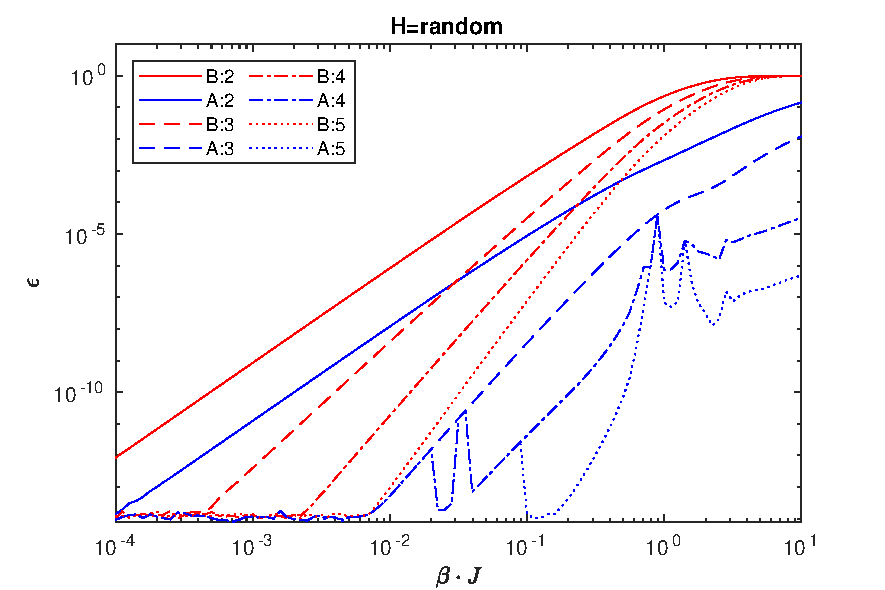
\includegraphics[width=\textwidth]{Figuren/benchmarking/rand_03.pdf}
%         \subcaption{test}
%     \end{subfigure}

%     \begin{subfigure}[]{\textwidth}
%         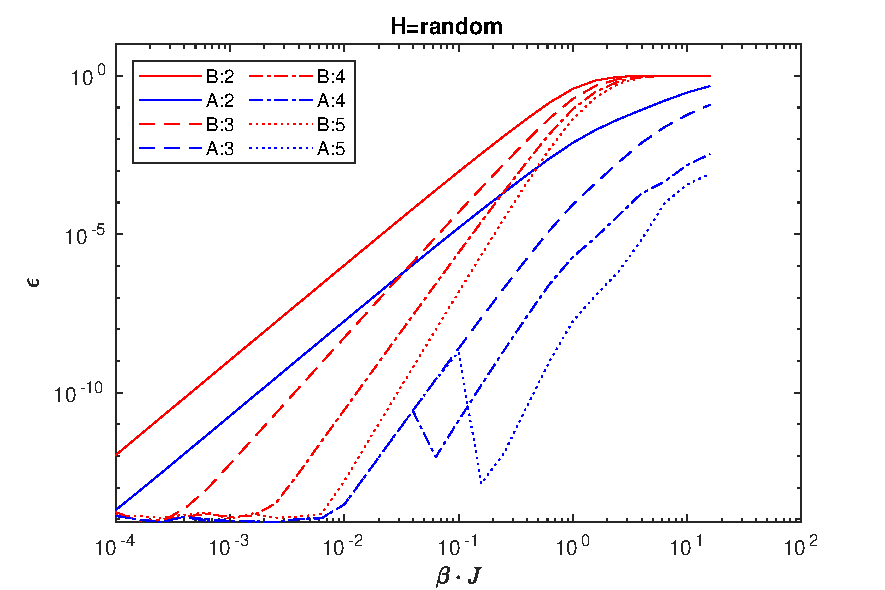
\includegraphics[width=\textwidth]{Figuren/benchmarking/rand_04.pdf}
%         \subcaption{test}
%     \end{subfigure}
%     \caption{test (cont.) }
%     \label{fig:benchmark:Random}
% \end{figure}

\subsection{Real time evolution} \label{subsec_rt_evo}

The method can also be used to construct real time evolution. \Cref{fig:benchmark:tising_time} shows the error of the matrix exponential in function of the time step $t = -i \beta $.

Also here, the results are promising. The construction handles complex matrices well. Similar to previous conclusion, type A performs better than type F, which performs better than type E.

The error of type A becomes quite large for high temperatures (not visible on figure), while type F keeps the errors low.

\begin{figure}
    \center
    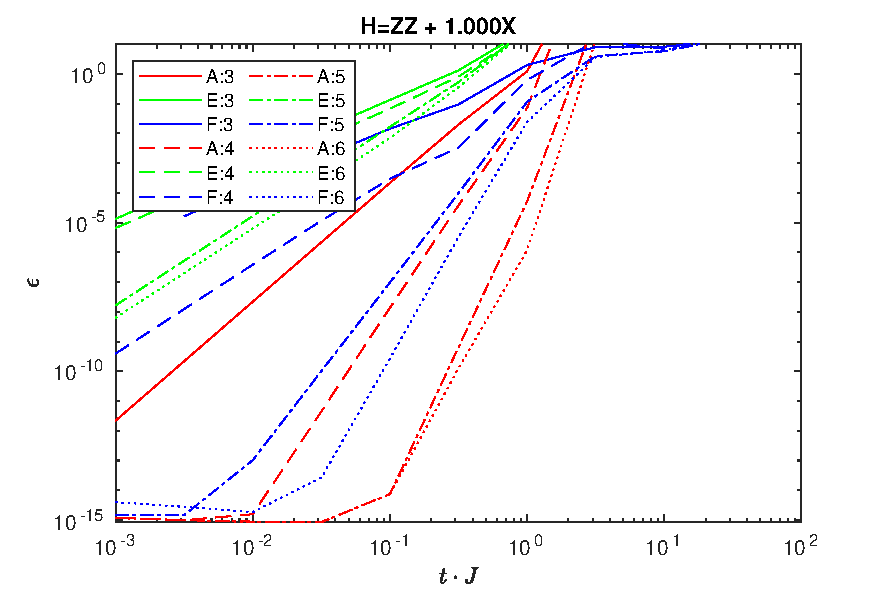
\includegraphics[width=\textwidth]{Figuren/benchmarking/1D_t_ising_time.pdf}
    \caption{Comparison type A, E and F for transversal Ising model. The horizontal axis represents the time step, not the inverse temperature. Virtual level 3 is truncated to $\chi=20$.  }
    \label{fig:benchmark:tising_time}
\end{figure}

This is not by any means a complete analysis of the real time evolution operator, but just a numeric example.

\subsection{Conclusion}

The biggest lesson, which took some time to figure out, was the correct way to implement the inversion procedure. It is essential that the pseudoinverse is taken for all the legs at once.
The different types were tested against each other, and it is clear that type A is clear that type A is better in almost all situations. The strict variants score worse. Type F keeps the inverses well-defined, and this shows at large $\beta$. Also, real time evolution works well.
The truncation procedure works as expected. A longer chain should not be constructed when a shorter chain was not solved fully (e.g. due to a truncation of the previous level)
Constructions with explicit rotation symmetry (see \cref{sec:symm}) perform exactly as good as the ones without.